\chapter{Upcoming plan}

TL;DR: Discuss shortly about the result, what we did not achieve and overview of the upcoming plan.

\section{The camera module}

After having discussed mainly the solutions and implementations of the soft modules in the system, we must move on to the main one that is considered to be the eyes of this thesis, which is the camera module. This section will discuss what parts are in a camera module and represent some images of a real one we built.

We can easily find the camera modules' parts from any retailer selling electrical components, robots, and Arduino kits. Additionally, in the current era of e-commerce, it is easier for us to find and compare those components that we need online. The parts required to build a camera module are listed below.

First, we need a camera part, and ESP32-CAM is the perfect one for this role. It is inexpensive and easy to use, making it ideal for our thesis that requires complex functions like image tracking and recognition. Furthermore, it integrates Wi-Fi, traditional Bluetooth, which help us in sending the images to the user's smartphone for the next steps in translating sign language.

Secondly, we need a converter adapter to help us sideload the program into the camera module. Besides, the third part that we need is the ultrasonic sensor mentioned in the TK section. It plays a role in location detection, which will tell the system the distance between hands and the camera module. Last but not least, this camera module needs a battery to power the whole module, and we reckon that the volume of about 100 mAh is fine.

Furthermore, there must be a box to store all the above parts. With the help of current 3D printing technology, we design that package on Tinkercad, an online 3D modeling program that runs on the web browser. After getting all the necessary components, we tried to put them all together and get the result below.

\begin{figure}[H]
  \centering
  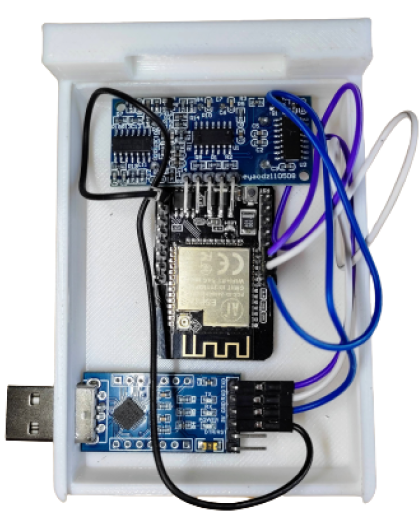
\includegraphics[width=0.45\textwidth]{img/Chap5/Prototype_View_inside.png}
  \caption{The components inside the camera module prototype}
\end{figure}

\begin{figure}[H]
  \centering
	\begin{subfigure}[b]{0.45\textwidth}
    \centering
    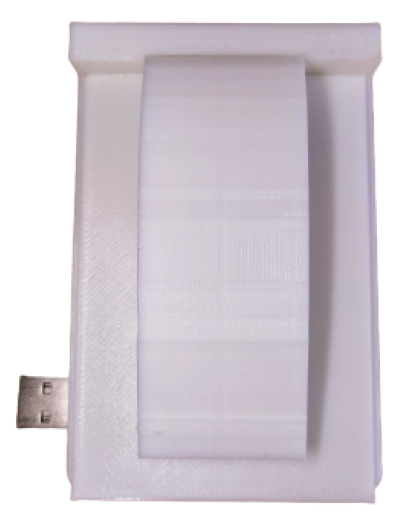
\includegraphics[width=\textwidth]{img/Chap5/Prototype_View_above.png}
  \end{subfigure}
  \hfill
	\begin{subfigure}[b]{0.46\textwidth}
    \centering
    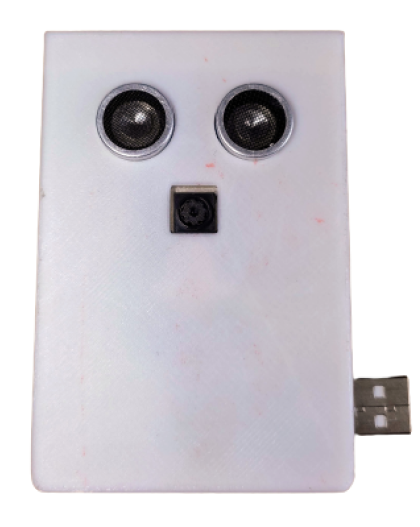
\includegraphics[width=\textwidth]{img/Chap5/Prototype_View_under.png}
  \end{subfigure}
	\caption{Views of the camera module prototype from the above and under}
\end{figure}

\begin{figure}[H]
  \centering
	\begin{subfigure}[b]{0.45\textwidth}
    \centering
    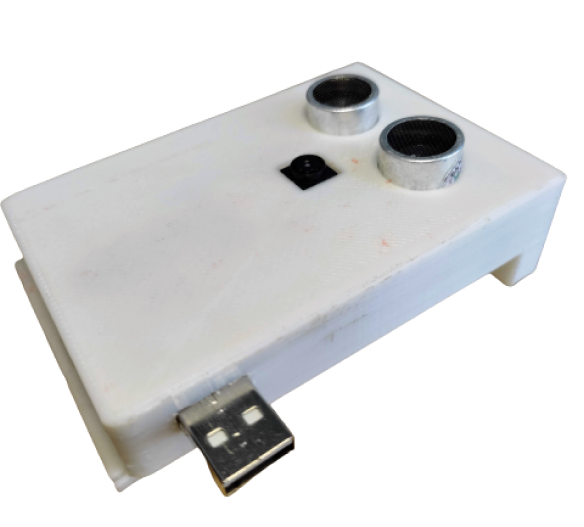
\includegraphics[width=\textwidth]{img/Chap5/Prototype_View_side_1.png}
  \end{subfigure}
  \hfill
	\begin{subfigure}[b]{0.45\textwidth}
    \centering
    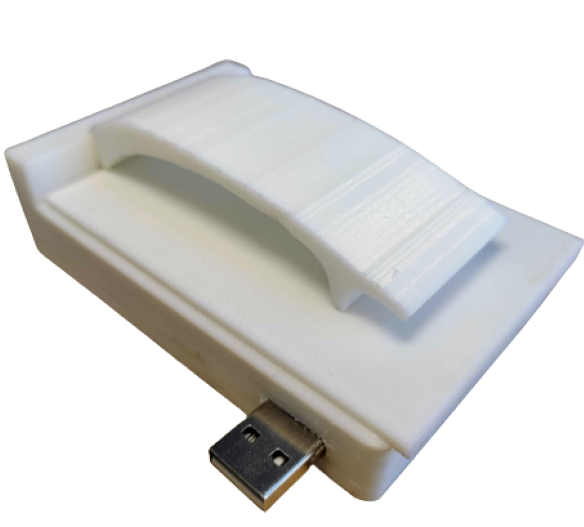
\includegraphics[width=\textwidth]{img/Chap5/Prototype_View_side_2.png}
  \end{subfigure}
	\caption{Views of the camera module prototype from the sides}
\end{figure}

Nevertheless, due to the smallest number that a 3D printer can print, the box's cover is a bit hard to put in. And the hanger that helped hang the box on the hat is not as flexible as we thought, so it needs a redesign.

\section{App building}

TODO: Put out the design from Figma

The current design of the application on the smartphone is considerably usable but not perfect, which means we need an upgrade in the design of the whole application in order to improve the user experience (UX) and user interface (UI).

\section{New features}

To expand the group of people using this application, we will implement additional features into the main application to help ordinary people learn and know more about sign language. Those features are a sign language dictionary and a learning system that help people learn sign language more efficiently. We will discuss more these two primary functions in the below subsections.

\subsection{Sign language dictionary}


\subsection{Learning system}

